\documentclass{article}
\textheight 23.5cm \textwidth 15.8cm
%\leftskip -1cm
\topmargin -1.5cm \oddsidemargin 0.3cm \evensidemargin -0.3cm
%\documentclass[final]{siamltex}

\usepackage{ctex}
\usepackage{verbatim}
\usepackage{fancyhdr}
\usepackage{graphicx}
\usepackage{amsmath}
\usepackage{amssymb}
\usepackage{float}
\usepackage{multirow}
\usepackage{colortbl}
\usepackage{amsthm}
\usepackage{bm}
\usepackage{tikz}

\textheight 23.5cm \textwidth 15.8cm
\topmargin -1.5cm \oddsidemargin 0.3cm \evensidemargin -0.3cm
\title{HW4 实验报告}
\author{PB20010429 侯相龙}

\begin{document}
\maketitle
\section{实验内容}
实现如下文章中 Seam Carving 算法:
Shai Avidan and Ariel Shamir. Seam Carving for Content-Aware Image Resizing. 
SIGGRAPH2007.


\section{实验原理}
Seam Carving算法是一种基于能量函数的图像缩放算法,其基本思想是在图像中寻找一条能量最小的路径,将该路径上的像素进行删除或插入操作,以达到图像缩放的效果。

该算法采用动态规划的思想,利用前一行的像素点路径来推导出当前行像素点路径的可能的最优解,从而找到能量最小的路径。
\section{算法介绍与步骤}
\begin{description}
    \item[1)]读入saliency图像,并将之转化为二维的能量矩阵。
    \item[2)]用动态规划算法找能量最小的缝。具体来说,若是求能量最低的竖直缝,采用bottom-up的方法计算前k行可能的最小代价(k从1到行数)
    最后求出可能的最小代价中的最小者,即为最小能量,根据动态规划表记录的索引可找到对应的缝
    \item[3)]若是增加/删减列,用2)中算法循环求能量最小的垂直缝并复制/删除相应的像素数据、能量矩阵的数据。
    \item[4)]若是增加/删减行,由于我们对像素数据的存储时行优先,这样做并不方便。可考虑对图像进行转置
    ,然后同3)增加/删减列即可。
    \item[5)] 返回修改后的像素数据。
\end{description}


\section{测试数据与实验结果}
原始的像素大小为500*324,修改后的大小见图。
% \begin{figure}[H]
%     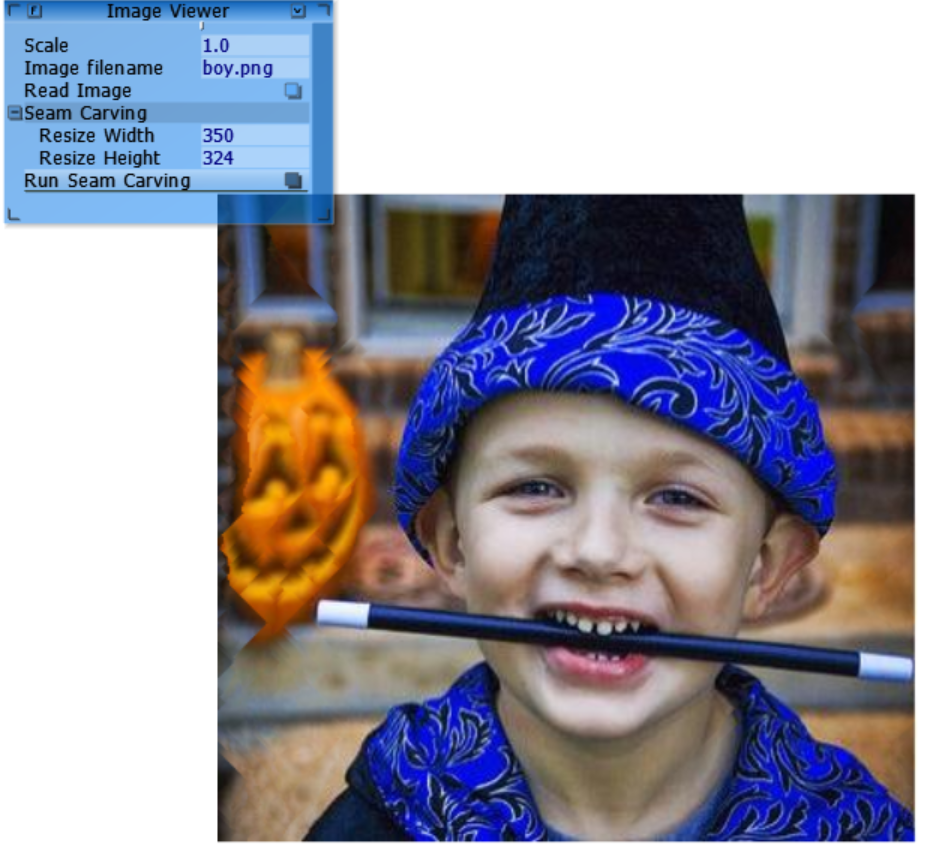
\includegraphics[width=0.4\textwidth]{1}
%     \caption{横向压缩:350*324}
%     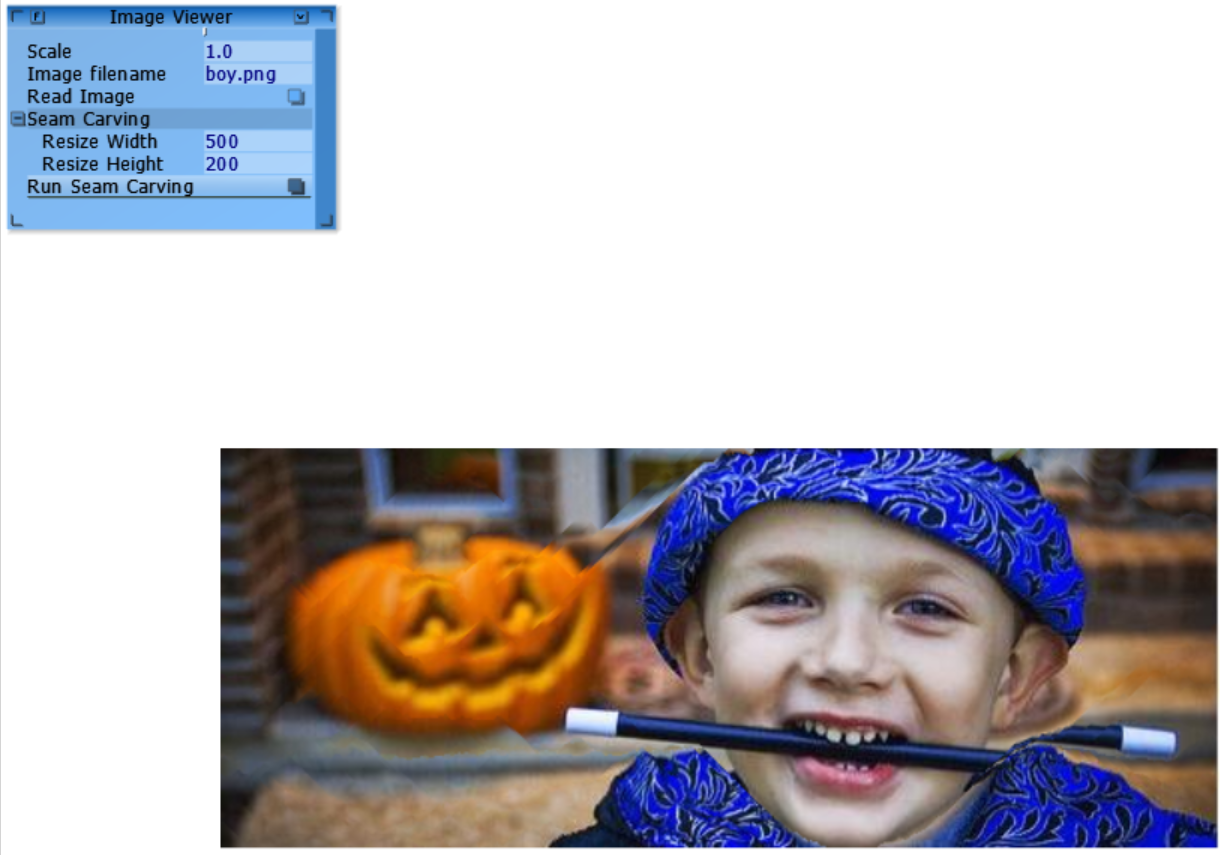
\includegraphics[width=0.4\textwidth]{2}
%     \caption{纵向压缩:500*200}

% \end{figure}

\begin{figure}[htbp]
    \centering
    \begin{minipage}[t]{0.4\linewidth}
      \centering
      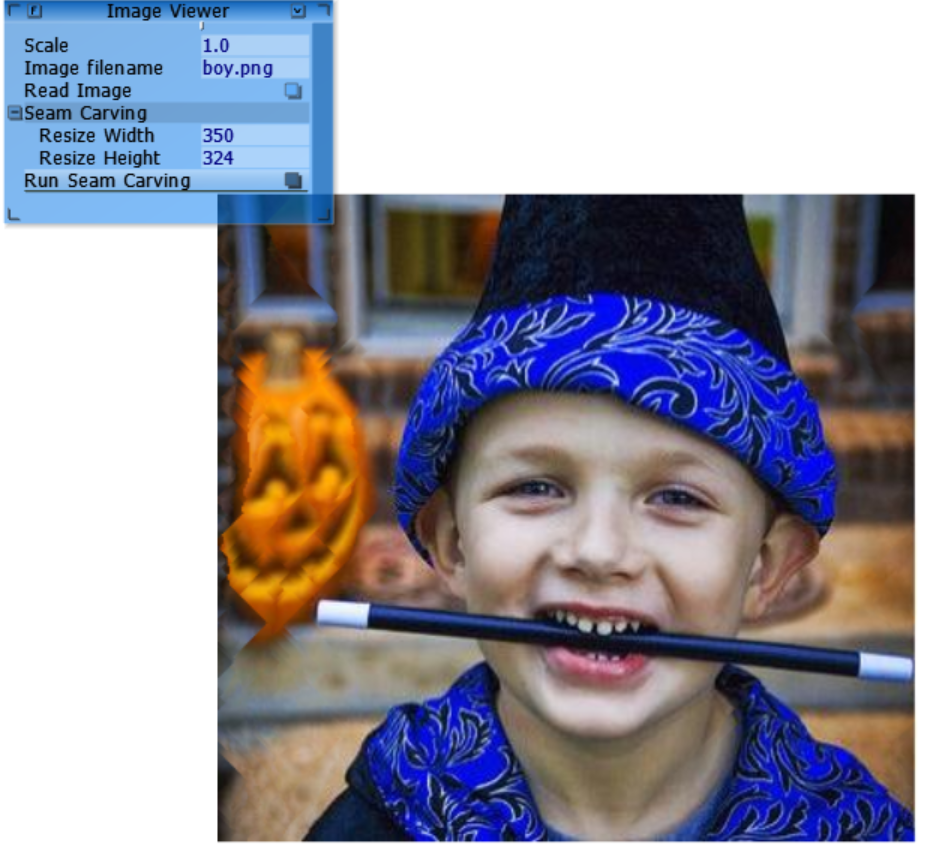
\includegraphics[width=\linewidth]{1.png}
      \caption{横向压缩:350*324}
      \label{fig:image1}
    \end{minipage}
    \hfill
    \begin{minipage}[t]{0.4\linewidth}
      \centering
      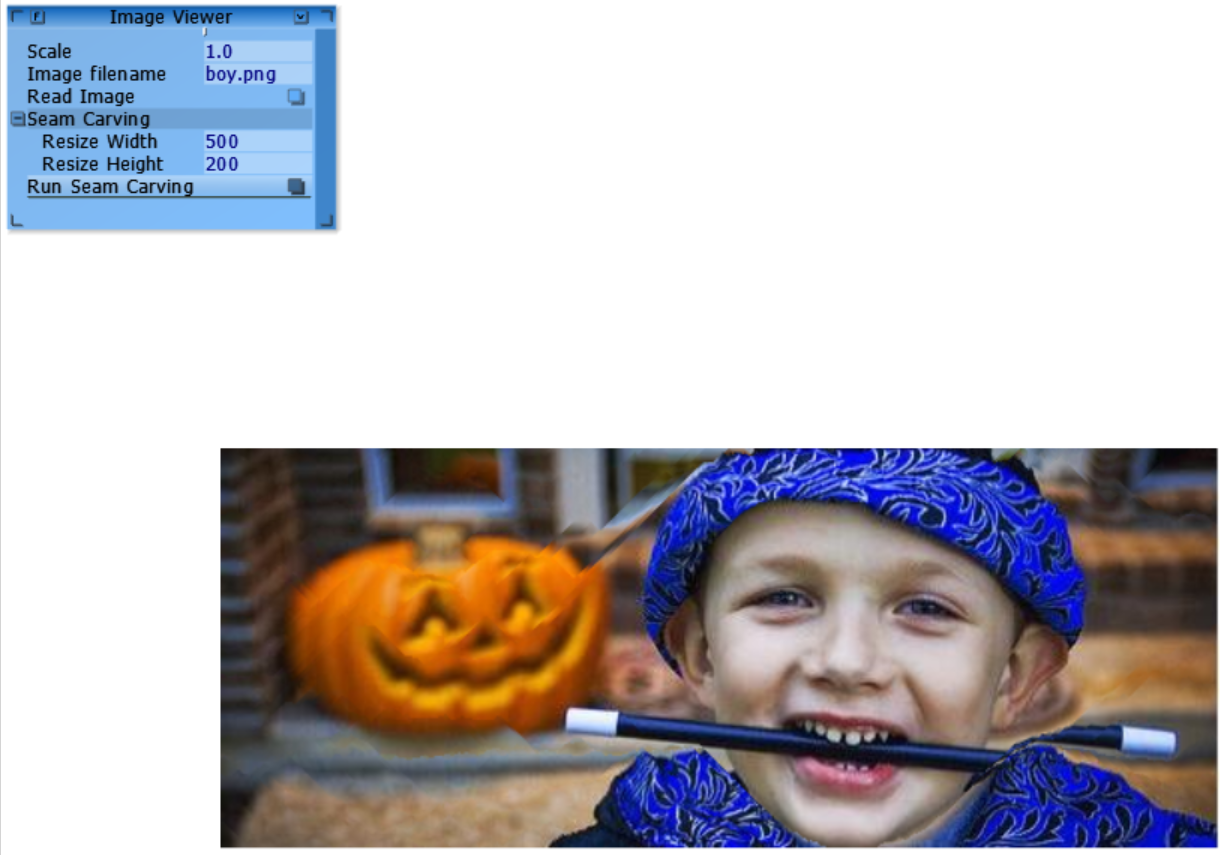
\includegraphics[width=\linewidth]{2.png}
      \caption{纵向压缩:500*200}
      \label{fig:image2}
    \end{minipage}

    \centering
    \begin{minipage}[t]{0.4\linewidth}
      \centering
      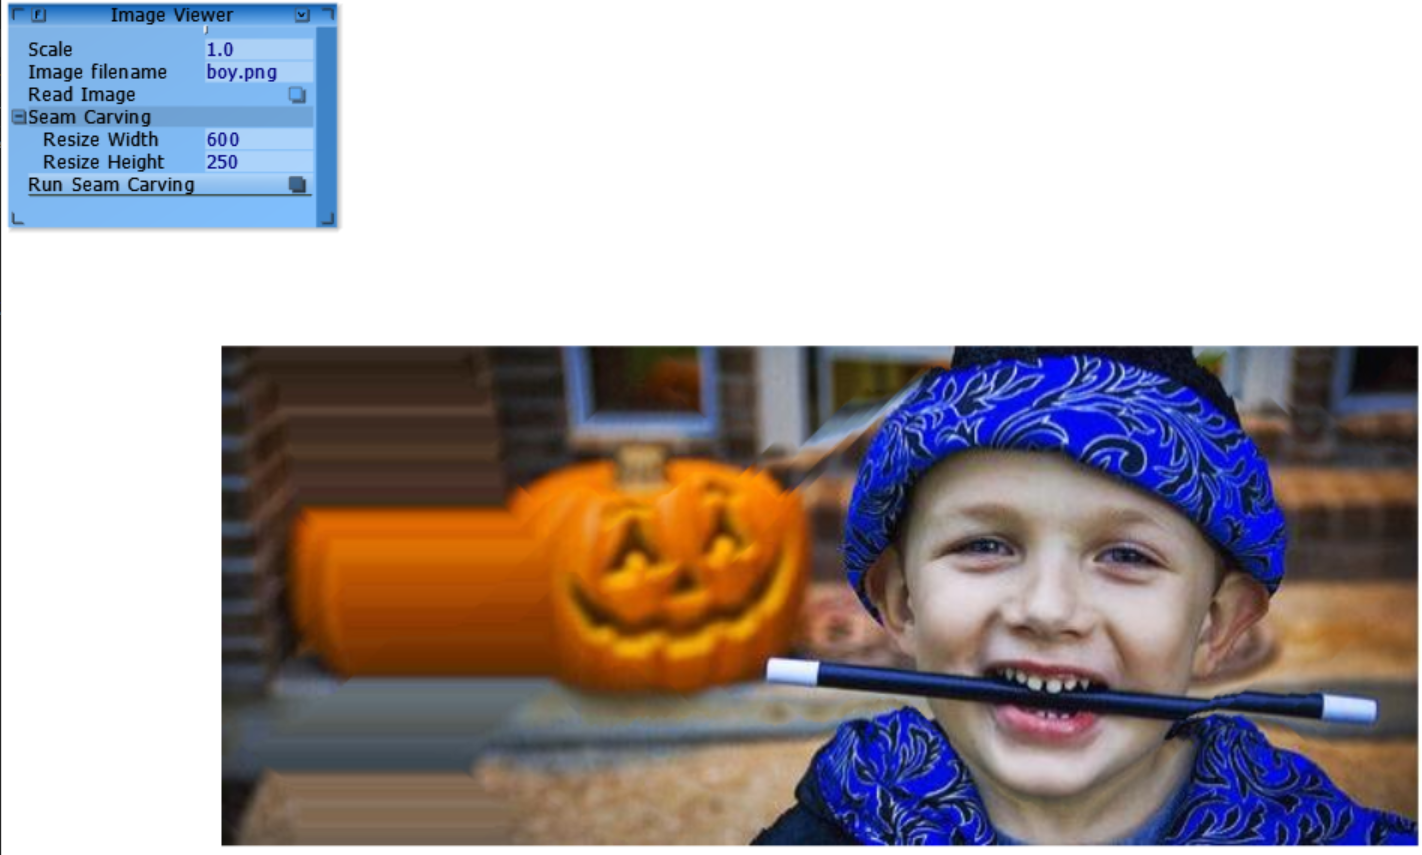
\includegraphics[width=\linewidth]{3.png}
      \caption{横纵同时变换:600*250}
      \label{fig:image3}
    \end{minipage}
    \hfill
    \begin{minipage}[t]{0.4\linewidth}
      \centering
      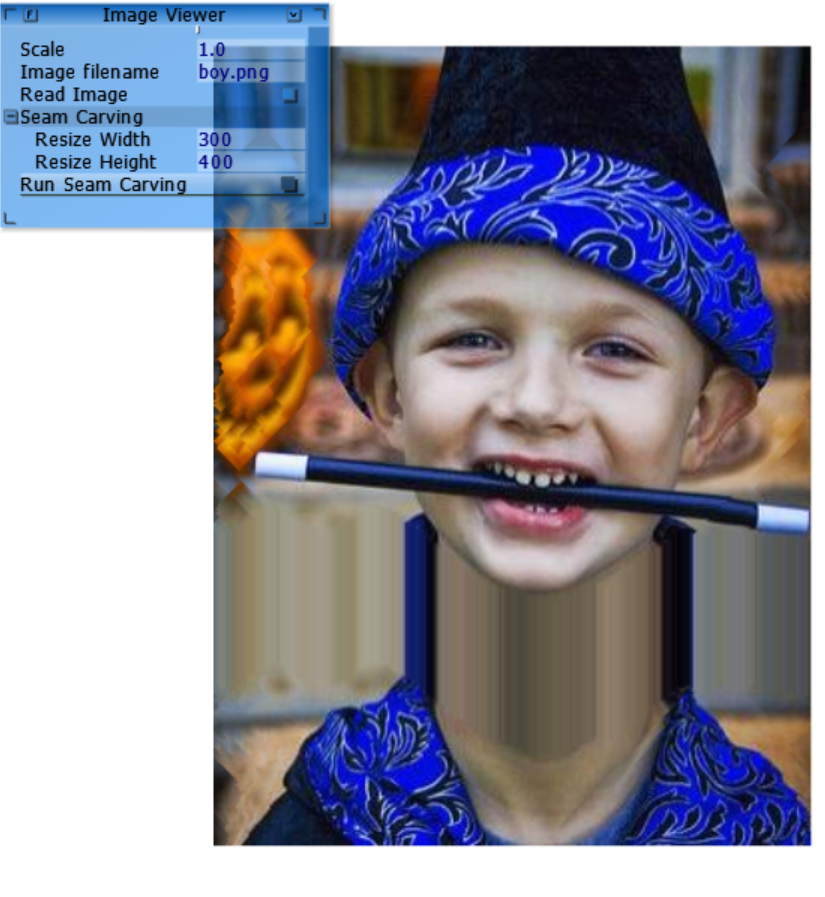
\includegraphics[width=\linewidth]{4.png}
      \caption{横纵同时变换:300*400}
      \label{fig:image4}
    \end{minipage}

  \end{figure}



\end{document}
